\documentclass{article}
\usepackage[utf8]{inputenc}
\usepackage[T1]{fontenc}
\usepackage[polish]{babel}
\usepackage{amsmath}
\usepackage{amssymb}
\usepackage{graphicx}
\begin{document}

\section*{Jan Mączyński, 344907}

\section*{RPiS - zad. nr 2}

\subsection*{Dane:}
rozwiązuję zadanie nr 3 - rozkład t-Studenta:
\[f(x) = \frac{\Gamma(\frac{k+1}{2})}{\sqrt{k\pi} \Gamma(\frac{k}{2})}
(1 + \frac{x^2}{k})^{-\frac{k+1}{2}},
\,k\in\mathbb{N},\,x\in\mathbb{R}\]
chcemy policzyć dystrybuantę
\[F(x) = \int_{-\infty}^{x} f(t)dt\]

\subsection*{Obliczanie funkcji $\Gamma-Eulera$}
we wzorze na $f(x)$ są dwa wystąpienia funkcji $\Gamma$:
\begin{itemize}
    \item $\Gamma(\frac{k+1}{2})$
    \item $\Gamma(\frac{k}{2})$
\end{itemize}
skoro $k\in\mathbb{N}$, to $k\in\mathbb{N}$, więc jako argumenty będą przyjmować
tylko liczby naturalne albo połówkowe (jak 1.5)\\\\
na ćwiczeniach udowodniliśmy następujące własności funkcji $\Gamma$:
\begin{itemize}
    \item $\Gamma(\frac{1}{2}) = \sqrt{\pi}$
    \item $\Gamma(p) = (p - 1)\Gamma(p - 1)$
    \item $\Gamma(z) = (z - 1)!,\,z\in\mathbb{Z}$
\end{itemize}
z pierwszych dwóch skorzystamy do obliczania wartości dla danych połówkowych,
a z ostatniej dla naturalnych

\subsection*{Obliczanie dystrybuanty}
$f(x)$ rozkładu t-Studenta jest funkcją parzystą, ponieważ jedyne wystąpienie
$x$ jest kwadratem ($x^2$), zatem $f(-x) = f(x)$\\\\
wiemy, że pole pod wykresem gęstości wynosi $1$, więc ze względu na symetrię pole połowy - dla $x\in(-\infty, 0]$ = $0.5$\\\\
teraz możemy rozbić obliczanie $F(x)$ na lepsze numerycznie (nie od $-\infty$) przypadki:
\begin{itemize}
    \item dla $x \geq 0$: całkujemy na przedziale $[0, x]$ i dodajemy lewą połowę (0.5):
        \[F(x) = 0.5 + \int_{0}^{x} f(t)dt\]
    \item dla $x \leq 0$: całkujemy na przedziale $[0, |x|]$ i odejmujemy:
        \[F(x) = 0.5 - \int_{0}^{|x|} f(t)dt\]
\end{itemize}

\subsection*{Obliczanie całki metodą Romberga}
aby obliczyć całkę $\int_0^{|x|} f(t) dt$ numerycznie najlepiej będzie wedle
sugestii skorzystać z metody Romberga (opratej na metodzie trapezów)

\subsubsection*{Złożony wzór trapezów}
ideą jest podzielenie obszaru całkowania $[a, b]$ (u nas [$0, |x|$]) na $n$
równych podprzedziałów o szerokości $h = \frac{b-a}{n}$ i przybliżenie funkcji
odcinkami między dokładnymi wartościami funkcji na krańcach przedziałów,
aby ostatecznie zsumować pola utworzonych trapezów\\
\begin{figure}[h]
    \centering
    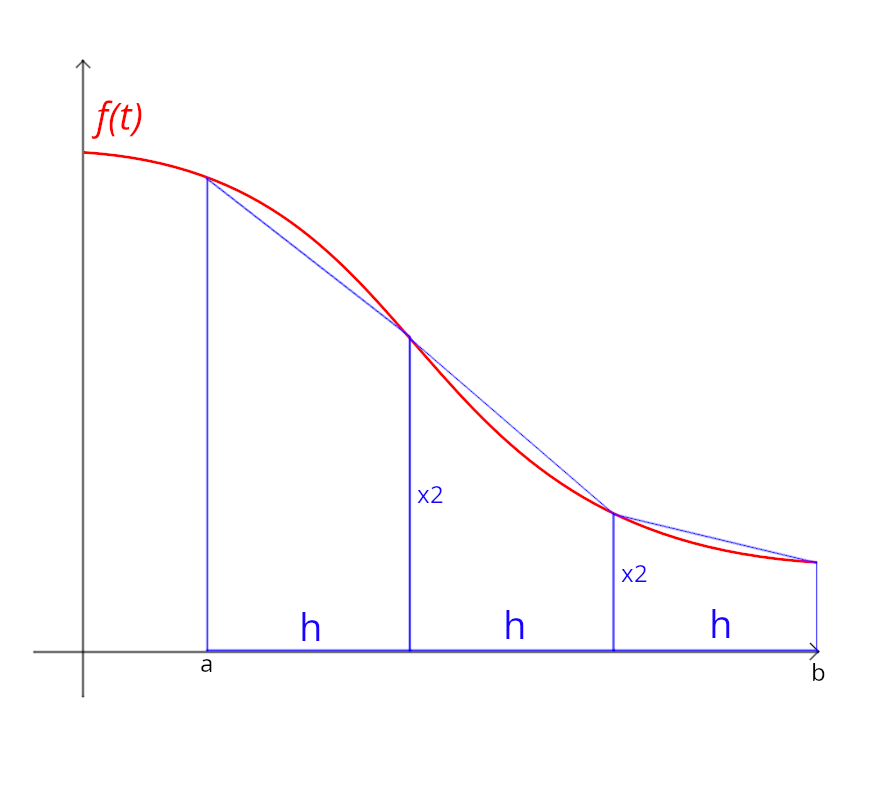
\includegraphics[width=0.5\textwidth]{trapezy.png}
\end{figure}
\\sumując ilości wystąpień funkcji $f$ we wzorze na pola trapezów otrzymujemy:
\[T(h) = \frac{h}{2} \left[ f(a) + 2\sum_{i=1}^{n-1} f(a + i \cdot h) + f(b) \right]\]
na zajęciach z Analizy Numerycznej sprawdziliśmy, że bład tej metody jest rzędu
$O(h^2)$, zatem zbiega stosunkowo wolno i możemy skorzystać z lepszej sposobu

\subsubsection*{Metoda Romberga}
aby przyspieszyć zbieżność skorzystamy z metody Romberga, o której również
była mowa na zajęciach z Analizy Numerycznej, polega ona na obliczaniu całki
wzorem trapezów dla coraz gęstszych podziałów (krok $h$ jest dzielony przez 2
w każdej iteracji), oraz kombinowaniu tych wyników w celu eliminacji błędów
niższych rzędów\\\\
proces ten tworzy tablicę (jak trójkąt) $R$, w której $R_{i,1}$ jest wynikiem
ze wzoru trapezów dla $2^{i-1}$ podprzedziałów, a wartości w kolejnych kolumnach
obliczane są za pomocą wzoru rekurencyjnego:
\[R_{i,j} = R_{i, j-1} + \frac{R_{i, j-1} - R_{i-1, j-1}}{4^{j-1} - 1},\,j > 1\]\\
\begin{figure}[h]
    \centering
    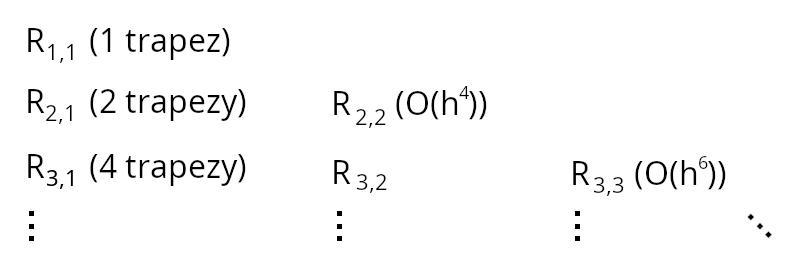
\includegraphics[width=0.5\textwidth]{romberg.png}
\end{figure}
\\rzędy błędu tej metody bardzo szybko maleją przesuwając się w prawy dół,
przy czym dokładamy stosunkowo mało wywołań $f(t)$

\end{document}
